\chapter{Operational parameter exploration and their implications}

\section{Introduction}

Building on the foundations laid by the preceding chapters, this chapter delves into a more nuanced investigation of the parametric influences on the resulting force curves obtained through Atomic Force Microscopy (AFM). When operating an AFM, it is typical to use a standard set of operational parameters. \cite{Schirmeisen2007} These parameters are often found during operation in an exploratory manner to find a good signal to noise ratio. However, it can be prudent  to examine a spectrum of force curves under varied conditions. Such an investigation enables the assessment of result consistency across diverse settings, thereby ensuring that the observed outcomes are not merely artifacts of parameter-specific minima phenomena. Additionally, a range of differing conditions can provide an insight into how other phenomena may have an effect on the observed behaviour of the curves.

A range of differing conditions were repeated with the following parameter changes: Tip speed, dwell time, solution pH and force mapping. 

\subsubsection{Tip Speed Variations}
The velocity of the AFM tip's approach and retraction impacts the force measurements, potentially altering the energy landscape of particle interactions. Varying the tip speed not only affects the kinetic parameters but also provides insight into time-dependent phenomena such as lubrication forces and simple viscous drag. The adjustment of the tip's velocity probes the dynamic response of the system, shedding light on the viscoelastic properties of the medium and the rate-dependent behavior of interparticle forces.

The previous results were taken at 0.5Hz, or a tip speed of 1$\mu$m/s. Two other speeds were used; 0.1Hz (0.2$\mu$m/s) and 2Hz (4$\mu$m/s). 0.1Hz was done exclusively on 10mM.

\subsubsection{Effect of Dwell Time}

The incorporation of a 5-second dwell time between the approach and retrace allows for the relaxation of the system and the establishment of equilibrium conditions in between movements, potentially revealing the subtleties of time-dependent interactions. The extended dwell time is expected to amplify phenomena such as capillary forces and hydration layers, which are often overshadowed by more dominant forces in quicker measurements.

\subsubsection{Solution pH Influence}

The pH of the colloidal solution is a determinant of the surface charge on the silica particles, which in turn modulates the force interactions observed. The variations in pH are expected to impact the electrical double layer, thereby influencing the force profiles and interaction potentials, while retaining the same force curve profile ranges as shown previously.

\subsubsection{Forcemapping for wide range site analysis}

Forcemapping, a method of tracking force-distance curves over a defined grid area, was employed to obtain a comprehensive understanding of the force distribution across the sample. This technique is useful in discerning how heterogenious the analysed surface is and provides a statistical interpretation of interparticle forces across a range of areas.

The exploration of these parameters serves not just as a methodical inquiry into the forces acting within colloidal dispersions, but also as a means to justify our approach to force curve analysis. The diversity of these conditions reflects the complex nature of the studied system and underscores the need for a comprehensive dataset that accurately represents the multifaceted nature of particle interactions.

The subsequent section presents the force distributions across our dataset, providing empirical evidence to the impact of these discussed factors. Finally, the section highlights the differences between the ``standard" dataset and the modified parameters.

\section{Tip speed analysis}

One of the differences between the different tip speeds was the data density. For faster speed less data was taken, while slower speeds had more data taken. This was due to the rate in which the AFM takes in data - the AFM was set to take in the maximum rate of data throughout the whole process. This was done to maximise the volume of data usable for the binning process (as seen in chapter 5). 

For 0.1 and 0.5Hz frequencies, the data recording rate was sufficient to the support the processing of the curves, while 2Hz had significantly less data volume, and required a more involved fitting, with generally a lower bitsize setting used in the script - increasing the noise in the averaged curve.

For each of the points, the tip speed increase was done after the initial reading, thus meaning that the sites can be directly compared across the standard dataset and this dataset (i.e. 0.5Hz dataset was recorded, then 2Hz was recorded right after in the same area).

% 0.6mM Section
\subsubsection*{0.6mM}
For 0.6mM only one site was recorded. Interestingly 0.6mM presented the highest recorded repulsive force across the entire dataset. Due to the lower data density, and the force cap set at around 12nN, there was a small window in which to fit the contact region, leading to a higher failure rate by the script for each movement. It is interesting to note that for this concentration the retract force histogram has no attractive force associated with the return movement, possibly indicating that higher speeds to not give the system enough time to relax towards an attractive profile, or that the electrostatic component decay is time dependant.
\begin{figure}[h!]
\centering
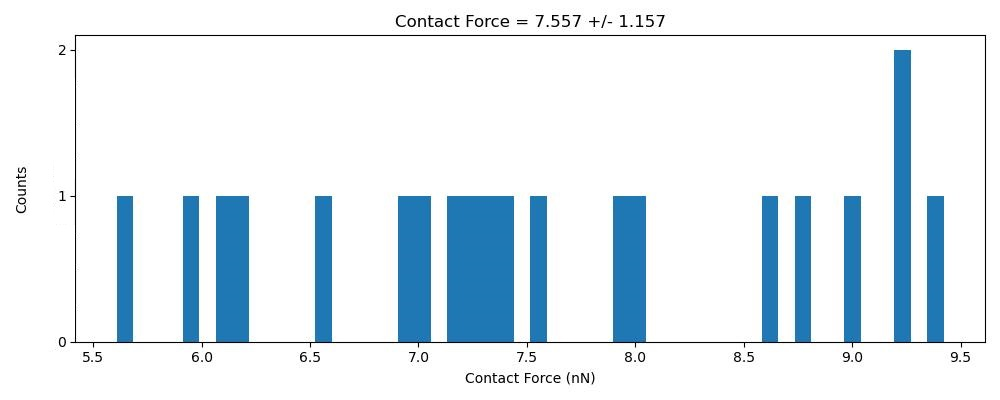
\includegraphics[width=\textwidth]{chapter7/Tip speed/0.6mM/approach_f_c_hist.jpg}
\caption{Approach force-current histogram at 0.6mM at 2Hz}
\end{figure}

\begin{figure}[h!]
\centering
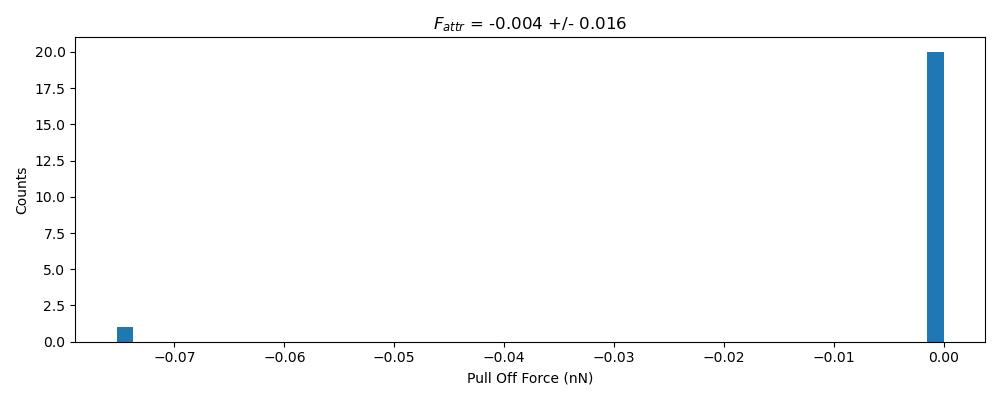
\includegraphics[width=0.9\textwidth]{chapter7/Tip speed/0.6mM/retract_f_a_hist.jpg}
\caption{Retract force-amplitude histogram at 0.6mM at 2Hz}
\end{figure}

\newpage

% 1.6mM Section
\subsubsection*{1.6mM}
1.6mM demonstrates a return to the previously expected values as set from the previous datasets. The retract curve demonstrates a widening of the attractive force, but still a very minor attraction.
\begin{figure}[h!]
\centering
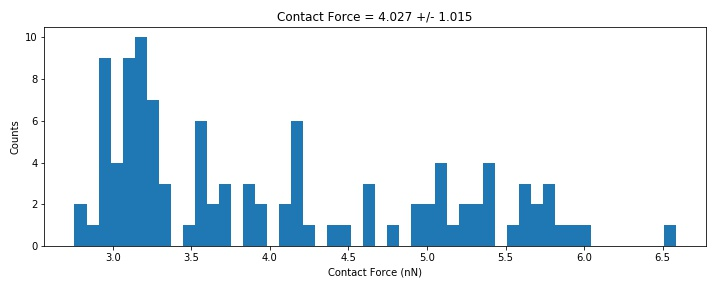
\includegraphics[width=.9\textwidth]{chapter7/Tip speed/1.6mM/S1 2Hz/approach_f_c_hist.jpg}
\caption{Approach curve for 1.6mM, S2 at 2Hz}
\end{figure}

\begin{figure}[h!]
\centering
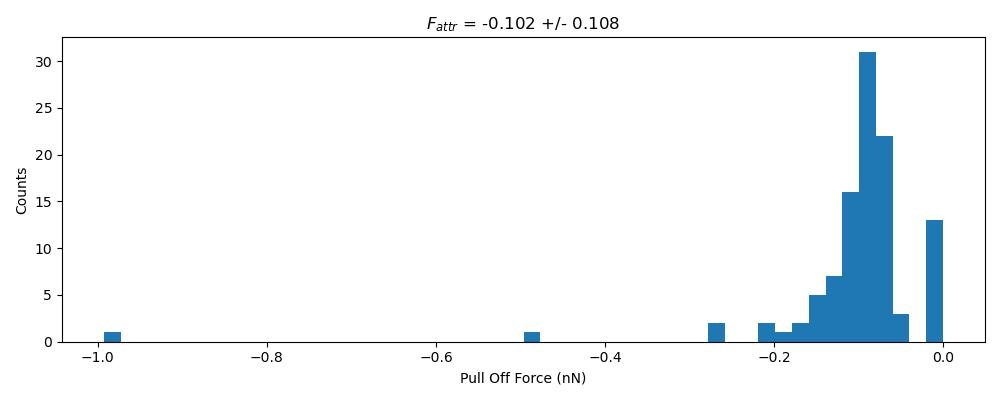
\includegraphics[width=.9\textwidth]{chapter7/Tip speed/1.6mM/S1 2Hz/retract_f_a_hist.jpg}
\caption{Retract curve for 1.6mM, S2 at 2Hz}
\end{figure}

\newpage

% 5mM Section
\subsubsection*{5mM}
5mM is the first concentration where a wider range of sites were explored. For the approach, the largest distribution was around the 2.5-4nN range, which is within expectations. For the retrace, minor instances of adhesive force was observed, but not significantly, again in line with previous results.

\begin{figure}[h!]
\paragraph{S1 2Hz}
\centering
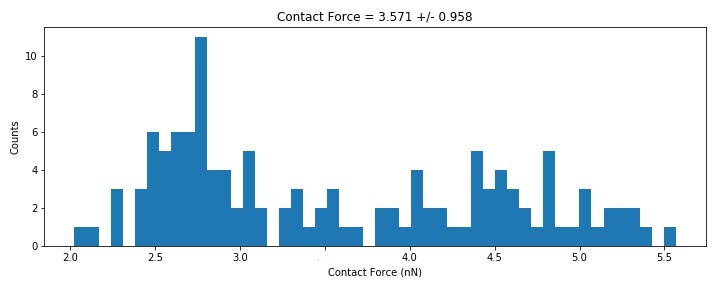
\includegraphics[width=\textwidth]{chapter7/Tip speed/5mM/S1 2Hz/approach_f_c_hist.jpg}
\caption{Approach curve for 5mM, S1 at 2Hz}
\end{figure}

\begin{figure}[h!]
\centering
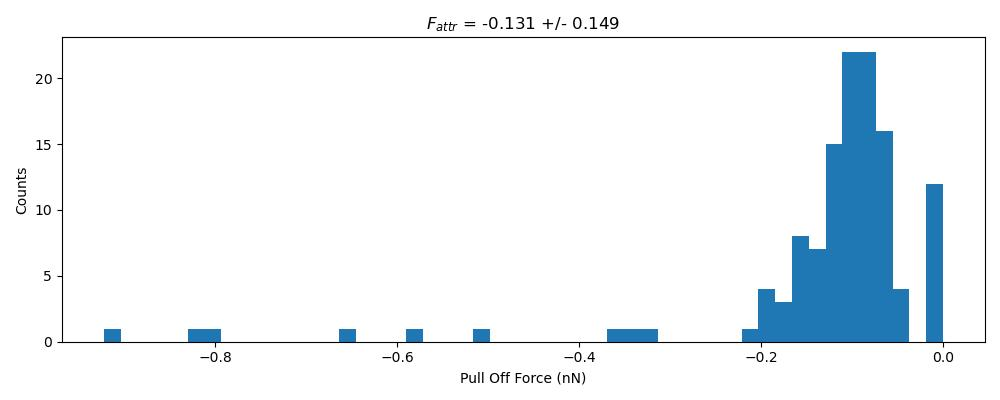
\includegraphics[width=\textwidth]{chapter7/Tip speed/5mM/S1 2Hz/retract_f_a_hist.jpg}
\caption{Retract curve for 5mM, S1 at 2Hz}
\end{figure}
\newpage


\begin{figure}[h!]
\paragraph{S2 2Hz}
\centering
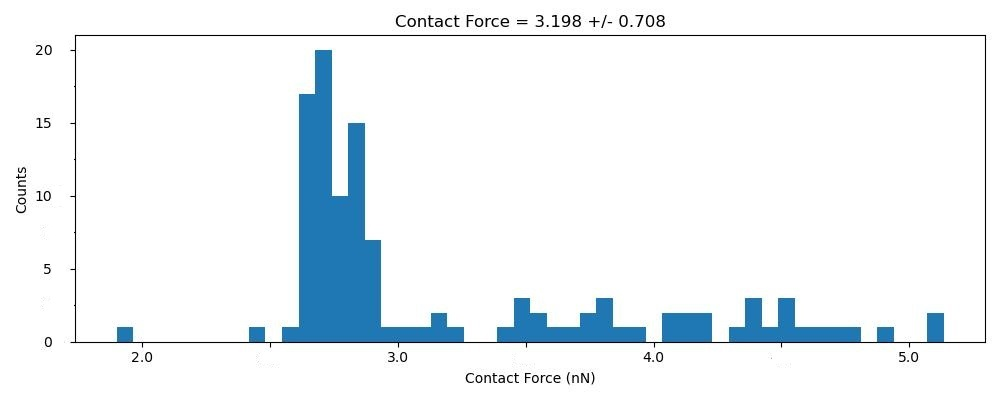
\includegraphics[width=\textwidth]{chapter7/Tip speed/5mM/S2 2Hz/approach_f_c_hist.jpg}
\caption{Approach curve for 5mM, S2 at 2Hz}
\end{figure}

\begin{figure}[h!]
\centering
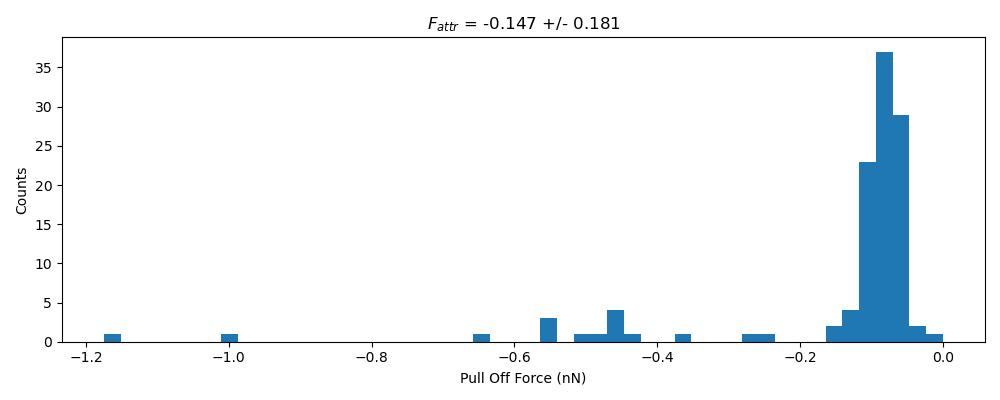
\includegraphics[width=\textwidth]{chapter7/Tip speed/5mM/S2 2Hz/retract_f_a_hist.jpg}
\caption{Retract curve for 5mM, S2 at 2Hz}
\end{figure}
\newpage


\begin{figure}[h!]
\paragraph{S3 2Hz}
\centering
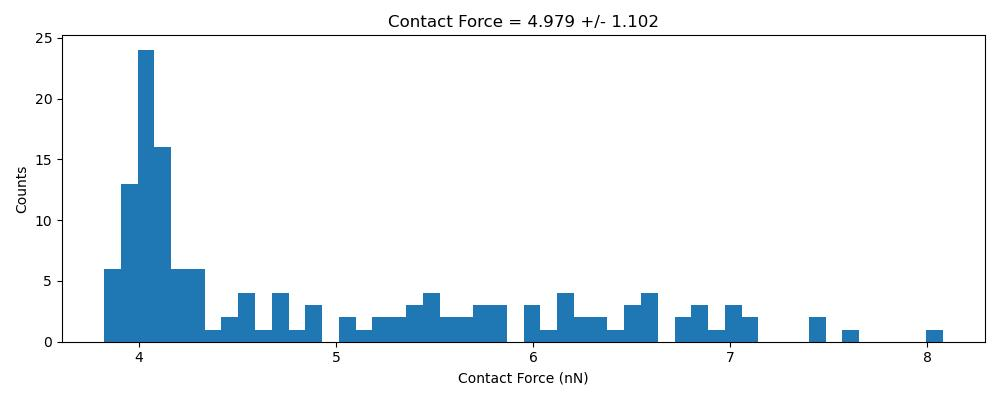
\includegraphics[width=\textwidth]{chapter7/Tip speed/5mM/S3 2Hz/approach_f_c_hist.jpg}
\caption{Approach curve for 5mM, S3 at 2Hz}
\end{figure}

\begin{figure}[h!]
\centering
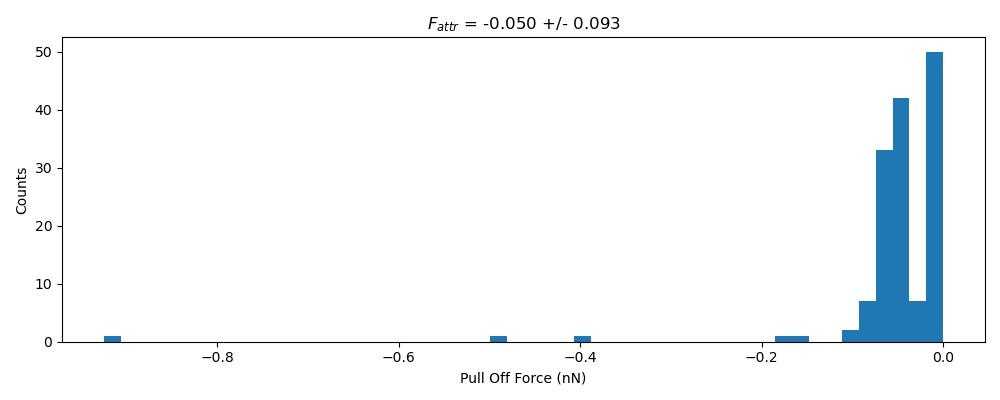
\includegraphics[width=\textwidth]{chapter7/Tip speed/5mM/S3 2Hz/retract_f_a_hist.jpg}
\caption{Retract curve for 5mM, S3 at 2Hz}
\end{figure}
\newpage

% 10mM Section
\subsubsection*{10mM}
10mM also includes an analysis of a slower tip - a tip speed of 0.1Hz. This was the only site to include a slower speed. Overall, for 0.1Hz, while 1 datapoint shows a significantly high attractive force, the other 2 largely show little to no attraction. Overall however, the 0.1Hz speed shows a slightly stronger retrace attractive force when compared to the previous data. 2Hz shows data within expected ranges from previous data.
\begin{figure}[h!]
\paragraph{S1 0.1Hz}
\centering
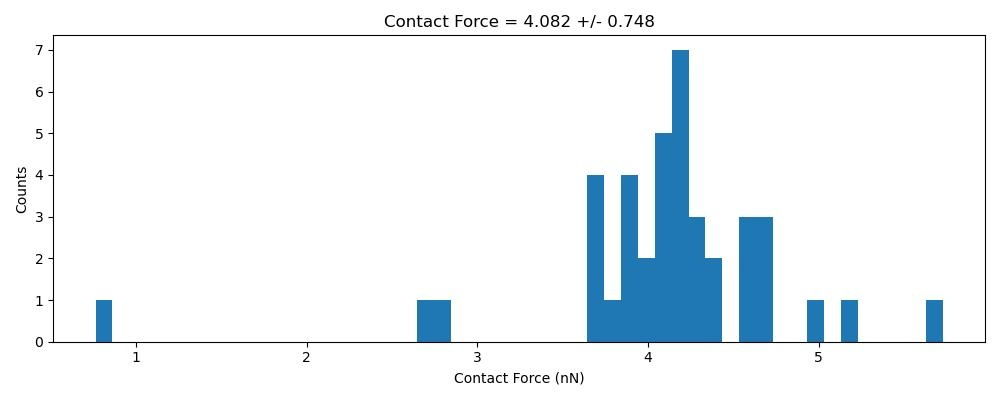
\includegraphics[width=\textwidth]{chapter7/Tip speed/10mM/S1 0.1Hz/approach_f_c_hist.jpg}
\caption{Approach curve for 10mM, S1 at 0.1Hz}
\end{figure}

\begin{figure}[h!]
\centering
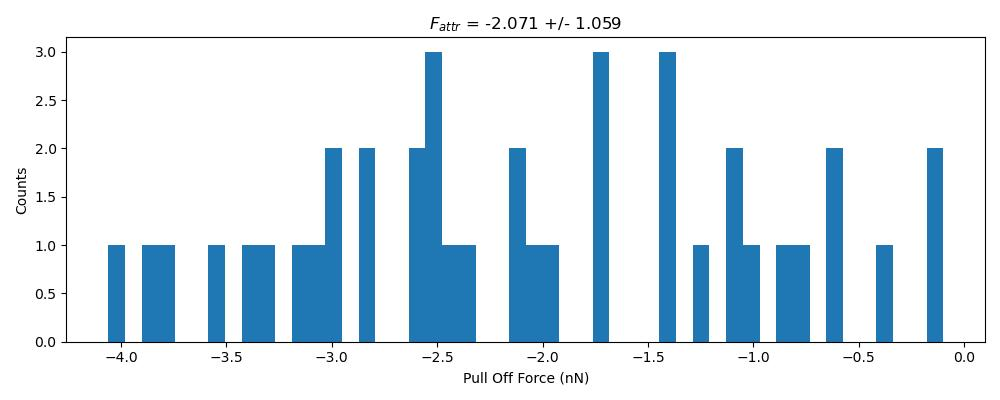
\includegraphics[width=\textwidth]{chapter7/Tip speed/10mM/S1 0.1Hz/retract_f_a_hist.jpg}
\caption{Retract curve for 10mM, S1 at 0.1Hz}
\end{figure}
\newpage

\begin{figure}[h!]
\paragraph{S1 2Hz}
\centering
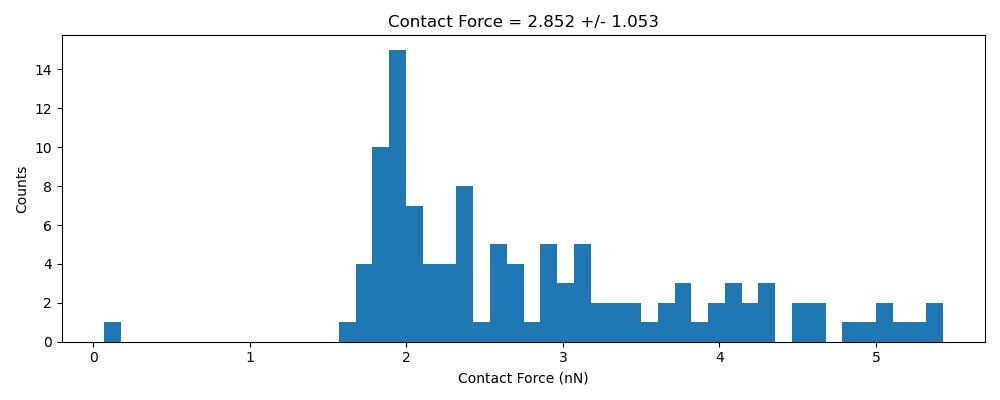
\includegraphics[width=\textwidth]{chapter7/Tip speed/10mM/S1 2Hz/approach_f_c_hist.jpg}
\caption{Approach curve for 10mM, S1 at 2Hz}
\end{figure}

\begin{figure}[h!]
\centering
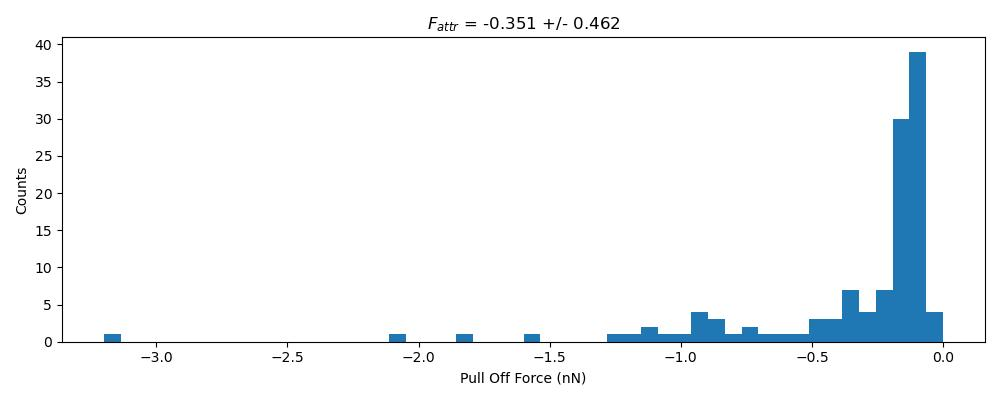
\includegraphics[width=\textwidth]{chapter7/Tip speed/10mM/S1 2Hz/retract_f_a_hist.jpg}
\caption{Retract curve for 10mM, S1 at 2Hz}
\end{figure}
\newpage


\begin{figure}[h!]
\paragraph{S2 0.1Hz}
\centering
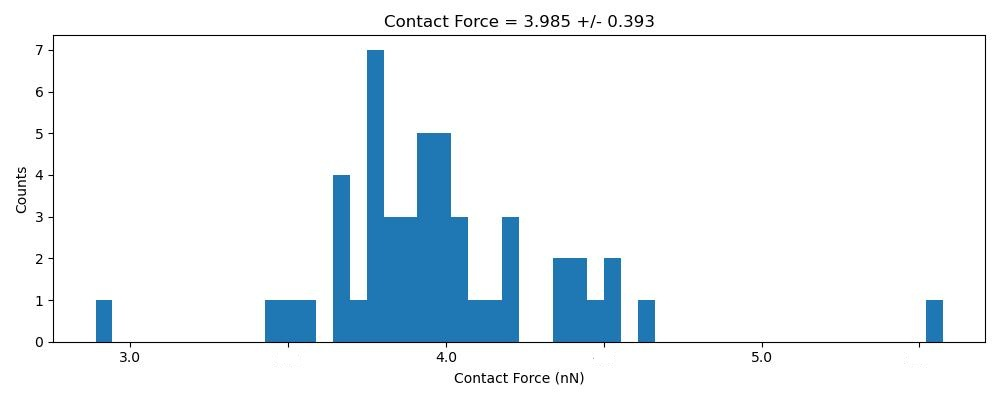
\includegraphics[width=\textwidth]{chapter7/Tip speed/10mM/S2 0.1Hz/approach_f_c_hist.jpg}
\caption{Approach curve for 10mM, S2 at 0.1Hz}
\end{figure}

\begin{figure}[h!]
\centering
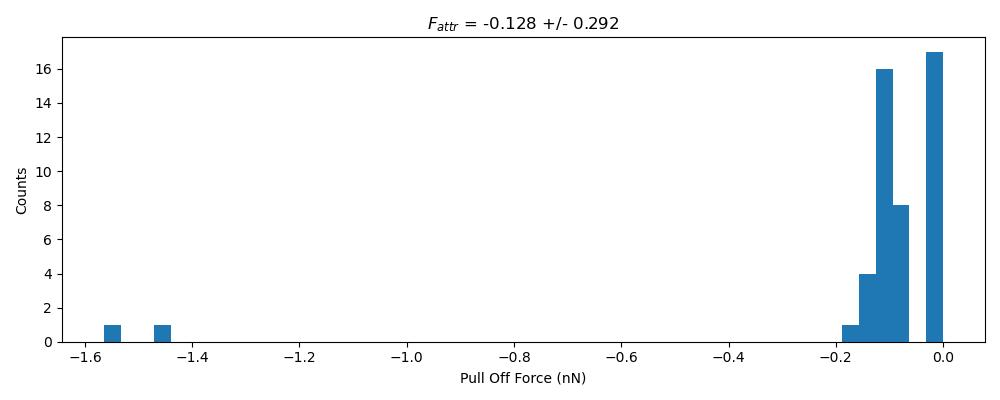
\includegraphics[width=\textwidth]{chapter7/Tip speed/10mM/S2 0.1Hz/retract_f_a_hist.jpg}
\caption{Retract curve for 10mM, S2 at 0.1Hz}
\end{figure}

\newpage


\begin{figure}[h!]
\paragraph{S2 2Hz}
\centering
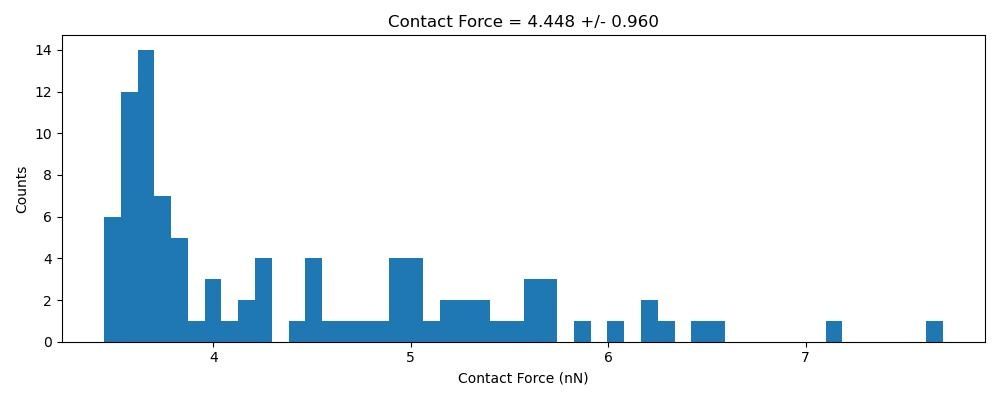
\includegraphics[width=\textwidth]{chapter7/Tip speed/10mM/S2 2Hz/approach_f_c_hist.jpg}
\caption{Approach curve for 10mM, S2 at 2Hz}
\end{figure}

\begin{figure}[h!]
\centering
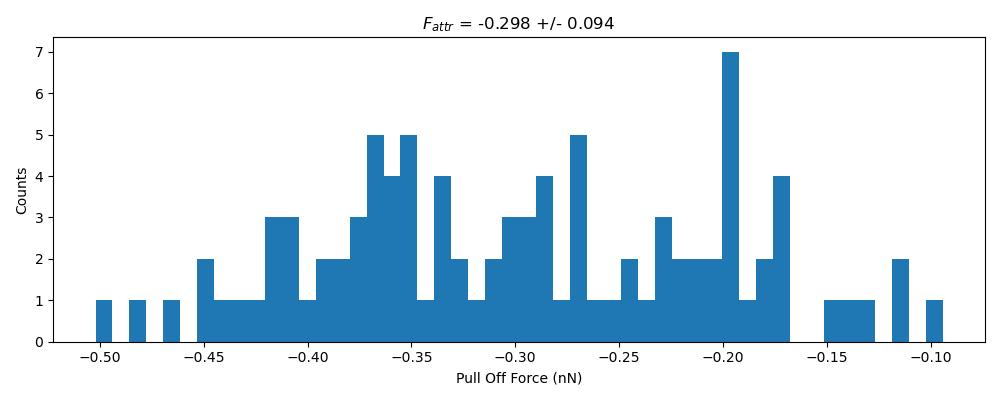
\includegraphics[width=\textwidth]{chapter7/Tip speed/10mM/S2 2Hz/retract_f_a_hist.jpg}
\caption{Retract curve for 10mM, S2 at 2Hz}
\end{figure}

\newpage


\begin{figure}[h!]
\paragraph{S3 0.1Hz}
\centering
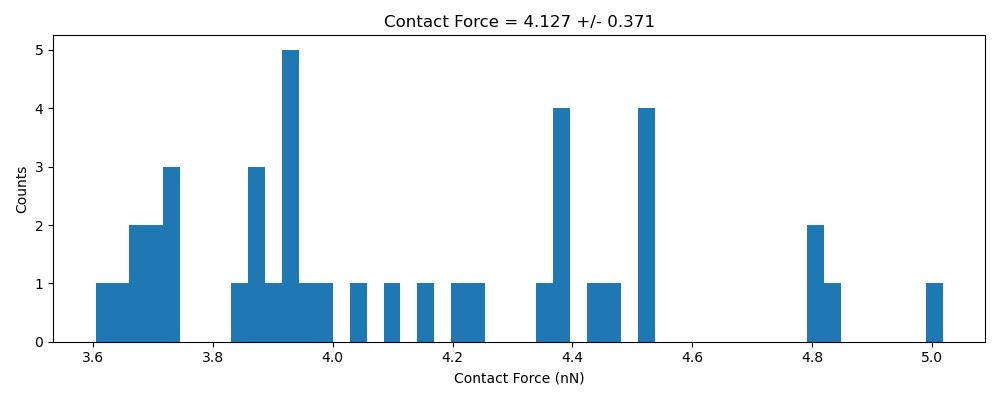
\includegraphics[width=\textwidth]{chapter7/Tip speed/10mM/S3 0.1Hz/approach_f_c_hist.jpg}
\caption{Approach curve for 10mM, S3 at 0.1Hz}
\end{figure}

\begin{figure}[h!]
\centering
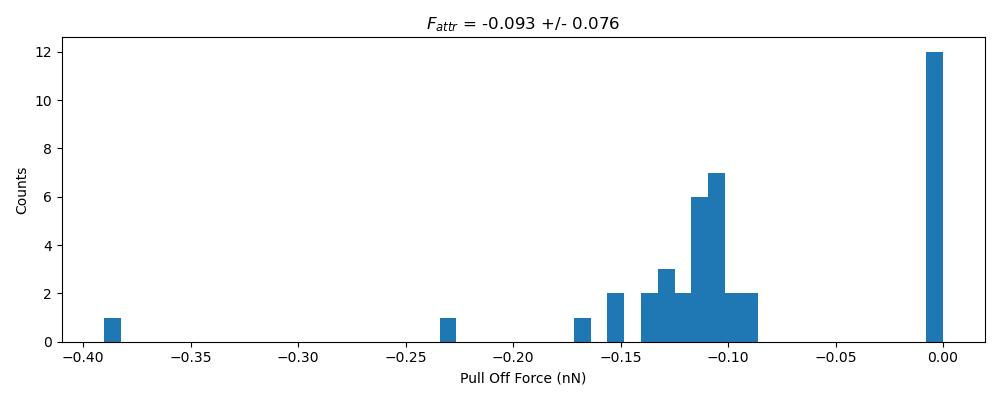
\includegraphics[width=\textwidth]{chapter7/Tip speed/10mM/S3 0.1Hz/retract_f_a_hist.jpg}
\caption{Retract curve for 10mM, S3 at 0.1Hz}
\end{figure}

\newpage


\begin{figure}[h!]
\paragraph{S3 2Hz}
\centering
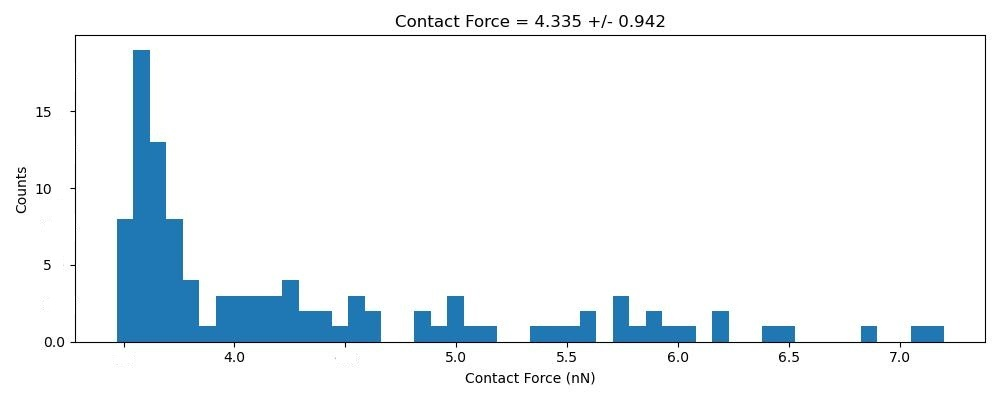
\includegraphics[width=\textwidth]{chapter7/Tip speed/10mM/S3 2Hz/approach_f_c_hist.jpg}
\caption{Approach curve for 10mM, S3 at 2Hz}
\end{figure}

\begin{figure}[h!]
\centering
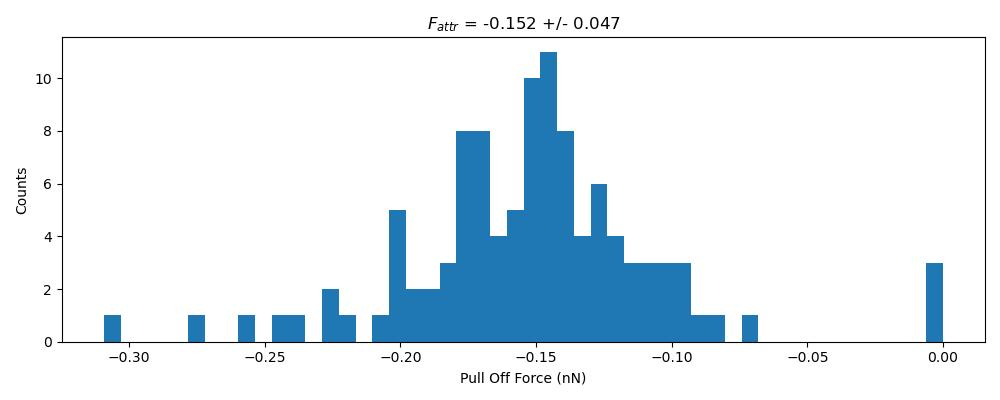
\includegraphics[width=\textwidth]{chapter7/Tip speed/10mM/S3 2Hz/retract_f_a_hist.jpg}
\caption{Retract curve for 10mM, S3 at 2Hz}
\end{figure}

\newpage

% 25mM Section
\subsubsection*{25mM}
25mM shows data within an expected range for the approach portion of the data, whereas the retrace demonstrates a significantly reduced attractive force. 
\begin{figure}[h!]
\paragraph{S1 2Hz}
\centering
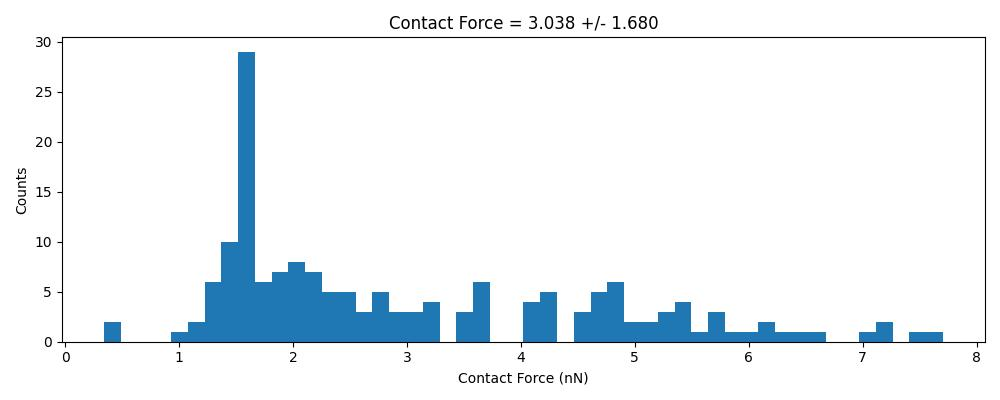
\includegraphics[width=\textwidth]{chapter7/Tip speed/25mM/S1 2Hz/approach_f_c_hist.jpg}
\caption{Approach curve for 25mM, S1 at 2Hz}
\end{figure}

\begin{figure}[h!]
\centering
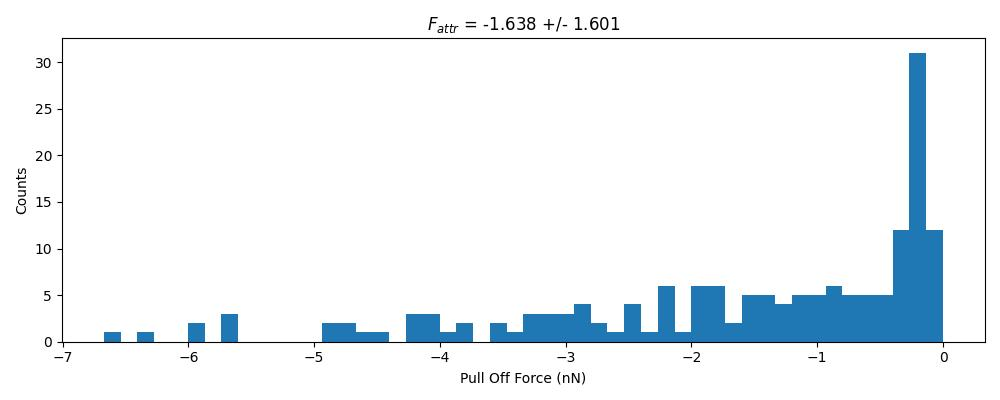
\includegraphics[width=\textwidth]{chapter7/Tip speed/25mM/S1 2Hz/retract_f_a_hist.jpg}
\caption{Retract curve for 25mM, S1 at 2Hz}
\end{figure}

\newpage


\begin{figure}[h!]
\paragraph{S2 2Hz}
\centering
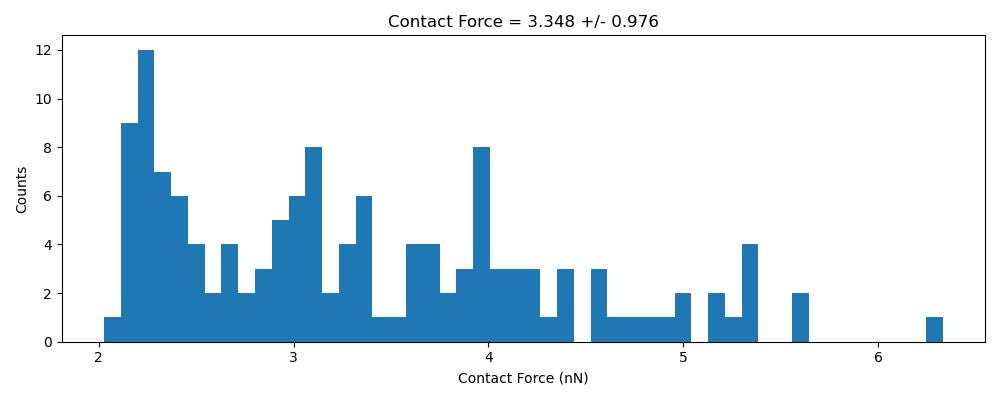
\includegraphics[width=\textwidth]{chapter7/Tip speed/25mM/S2 2Hz/approach_f_c_hist.jpg}
\caption{Approach curve for 25mM, S2 at 2Hz}
\end{figure}

\begin{figure}[h!]
\centering
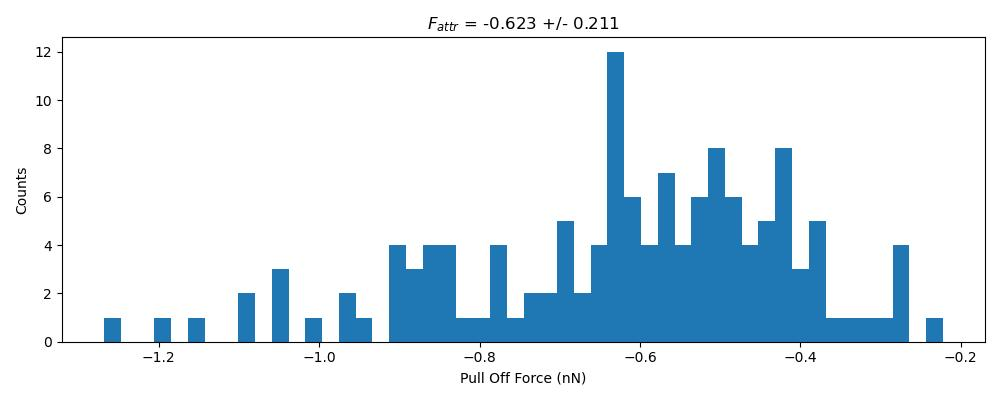
\includegraphics[width=\textwidth]{chapter7/Tip speed/25mM/S2 2Hz/retract_f_a_hist.jpg}
\caption{Retract curve for 25mM, S2 at 2Hz}
\end{figure}

\newpage


\begin{figure}[h!]
\paragraph{S3 2Hz}
\centering
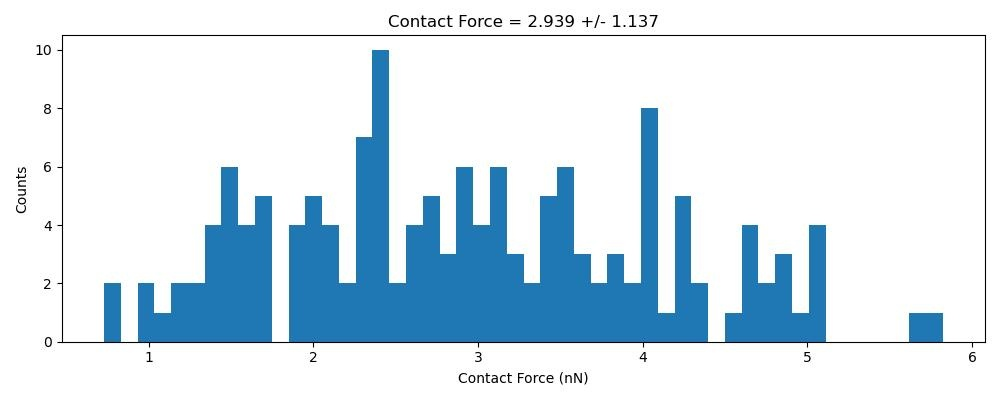
\includegraphics[width=\textwidth]{chapter7/Tip speed/25mM/S3 2Hz/approach_f_c_hist.jpg}
\caption{Approach curve for 25mM, S3 at 2Hz}
\end{figure}

\begin{figure}[h!]
\centering
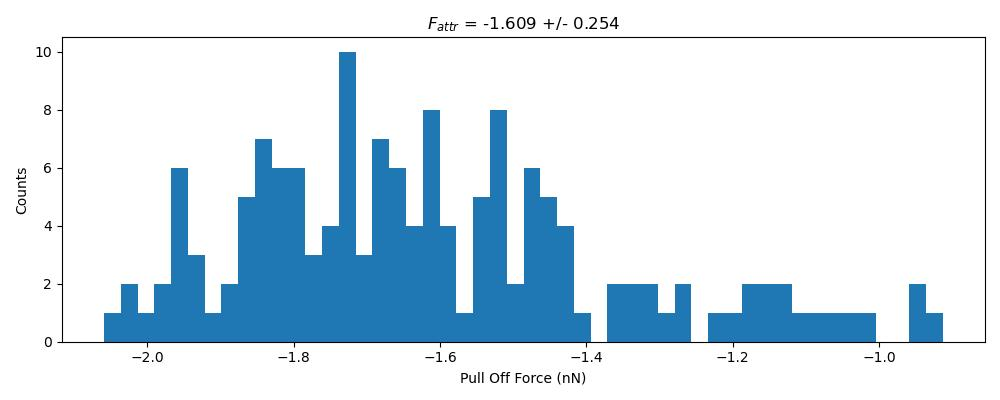
\includegraphics[width=\textwidth]{chapter7/Tip speed/25mM/S3 2Hz/retract_f_a_hist.jpg}
\caption{Retract curve for 25mM, S3 at 2Hz}
\end{figure}

\newpage

% 230mM Section
\subsubsection*{230mM}
230mM 2Hz again shows data within expected ranges, while having a slightly higher approach repulsive force. For the retrace attractive force, the results are similar, again with a slightly lower attractive force.
\begin{figure}[h!]
\paragraph{S1 2Hz}
\centering
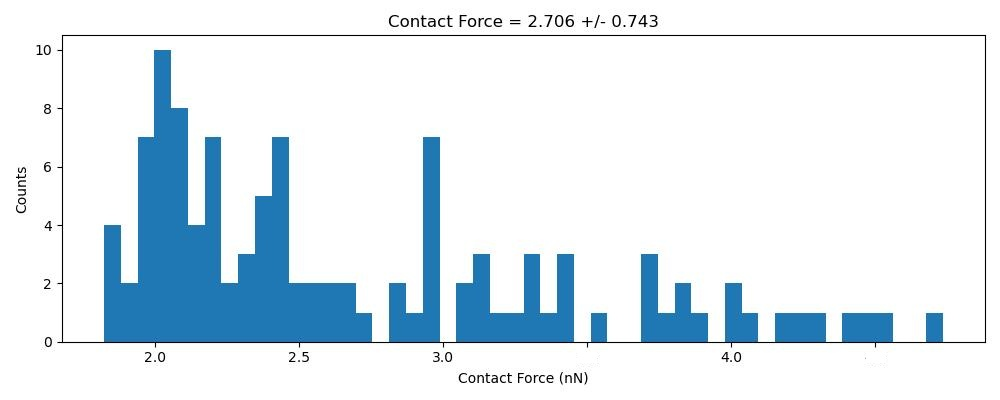
\includegraphics[width=\textwidth]{chapter7/Tip speed/230mM/S1 2Hz/approach_f_c_hist.jpg}
\caption{Approach curve for 230mM, S1 at 2Hz}
\end{figure}

\begin{figure}[h!]
\centering
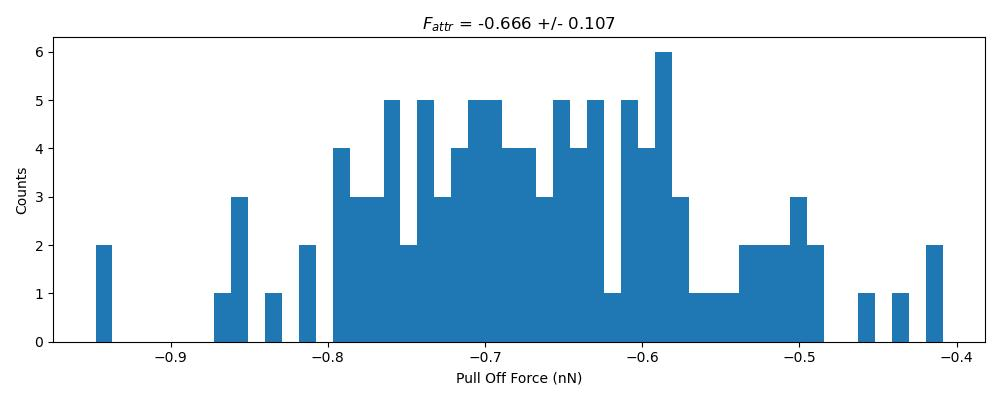
\includegraphics[width=\textwidth]{chapter7/Tip speed/230mM/S1 2Hz/retract_f_a_hist.jpg}
\caption{Retract curve for 230mM, S1 at 2Hz}
\end{figure}

\newpage


\begin{figure}[h!]
\paragraph{S2 2Hz}
\centering
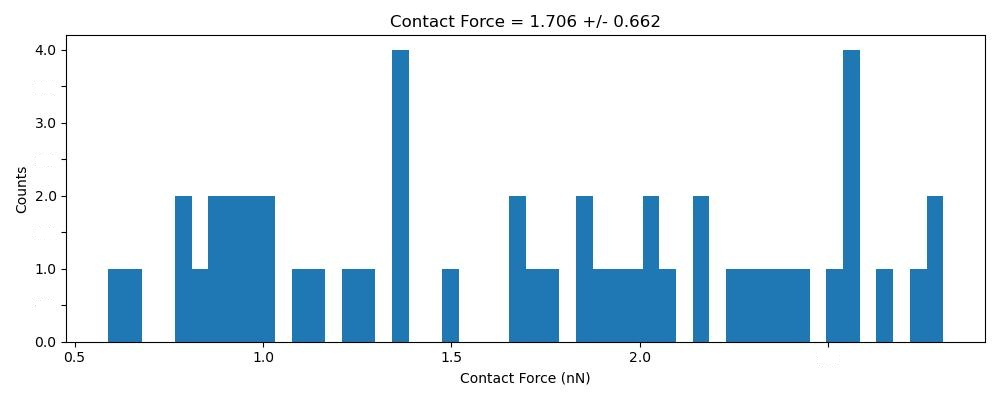
\includegraphics[width=\textwidth]{chapter7/Tip speed/230mM/S2 2Hz/approach_f_c_hist.jpg}
\caption{Approach curve for 230mM, S2 at 2Hz}
\end{figure}

\begin{figure}[h!]
\centering
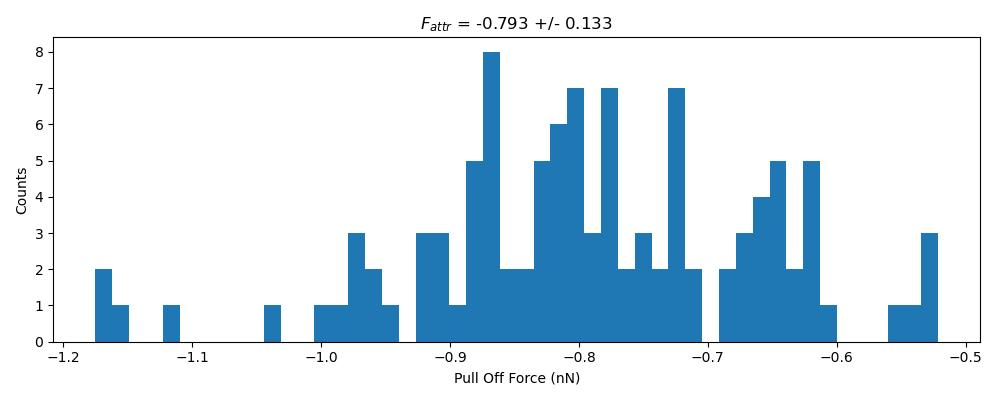
\includegraphics[width=\textwidth]{chapter7/Tip speed/230mM/S2 2Hz/retract_f_a_hist.jpg}
\caption{Retract curve for 230mM, S2 at 2Hz}
\end{figure}

\newpage

% 550mM Section
\subsubsection*{550mM}
550mM 2Hz marks a shift in approach forces towards the attractive. The results are similar again to other datapoints in this series; minorly reduced attractive force on the retrace. However, interestingly, the approach has very little attractive force. 
\begin{figure}[h!]
\paragraph{S2 2Hz}
\centering
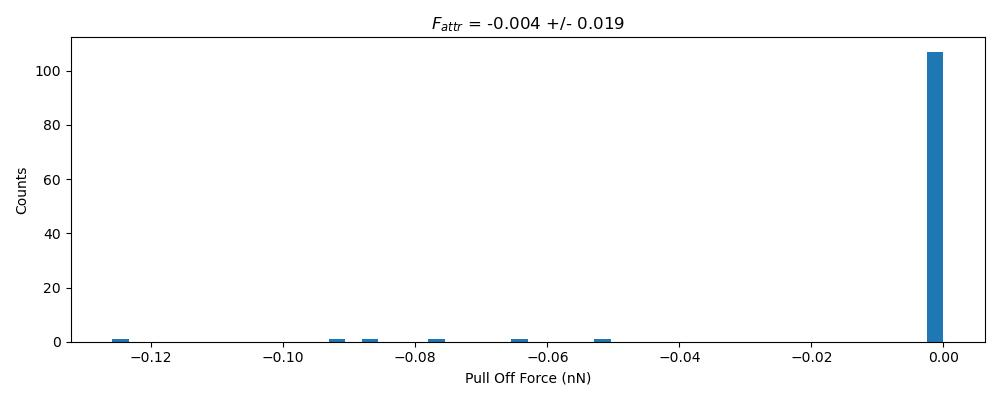
\includegraphics[width=\textwidth]{chapter7/Tip speed/550mM/S2 2Hz/approach_f_a_hist.jpg}
\caption{Approach curve for 550mM, S2 at 2Hz}
\end{figure}

\begin{figure}[h!]
\centering
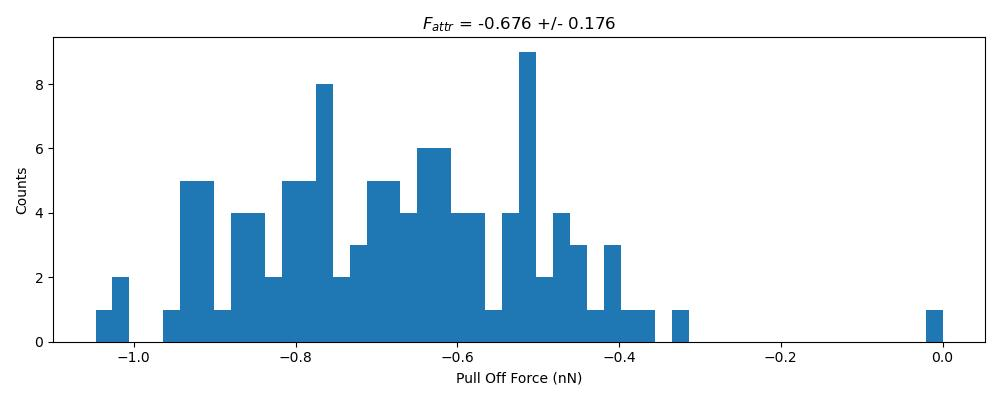
\includegraphics[width=\textwidth]{chapter7/Tip speed/550mM/S2 2Hz/retract_f_a_hist.jpg}
\caption{Retract curve for 550mM, S2 at 2Hz}
\end{figure}


\begin{figure}[h!]
\paragraph{S3 2Hz}
\centering
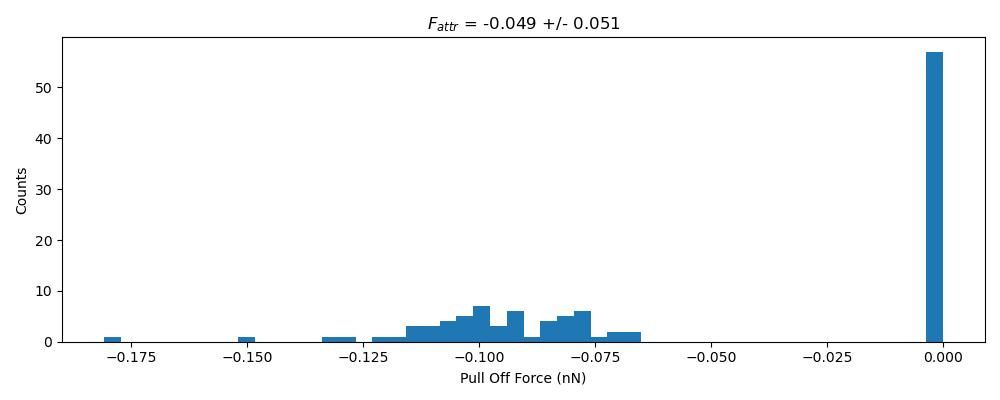
\includegraphics[width=\textwidth]{chapter7/Tip speed/550mM/S3 2Hz/approach_f_a_hist.jpg}
\caption{Approach curve for 550mM, S3 at 2Hz}
\end{figure}

\begin{figure}[h!]
\centering
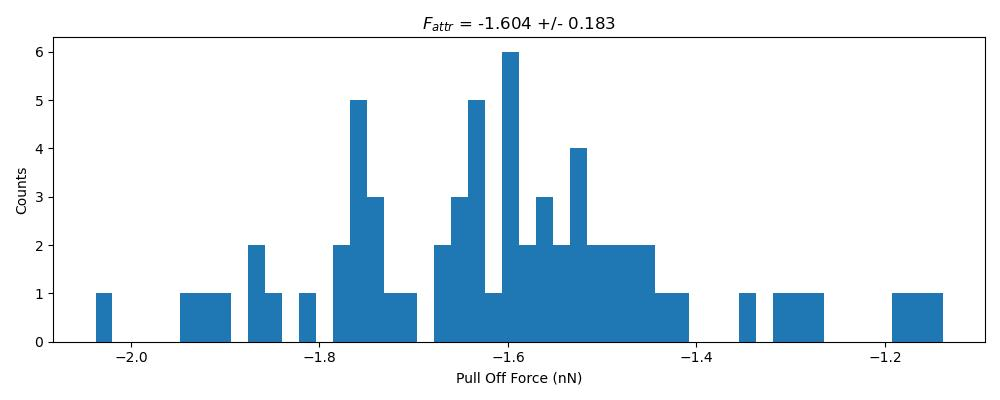
\includegraphics[width=\textwidth]{chapter7/Tip speed/550mM/S3 2Hz/retract_f_a_hist.jpg}
\caption{Retract curve for 550mM, S3 at 2Hz}
\end{figure}
\newpage

\subsubsection{Averaged curve of data}
These datapoints were then averaged, with the standard deviations ($Stdev_{avg}$) concatenated between sites using equation \ref{eq:Stdevavg}

These points were then plotted against the original dataset to investigate if any noticeable overall differences between points could be discerned.

\begin{figure}[h!]
\centering
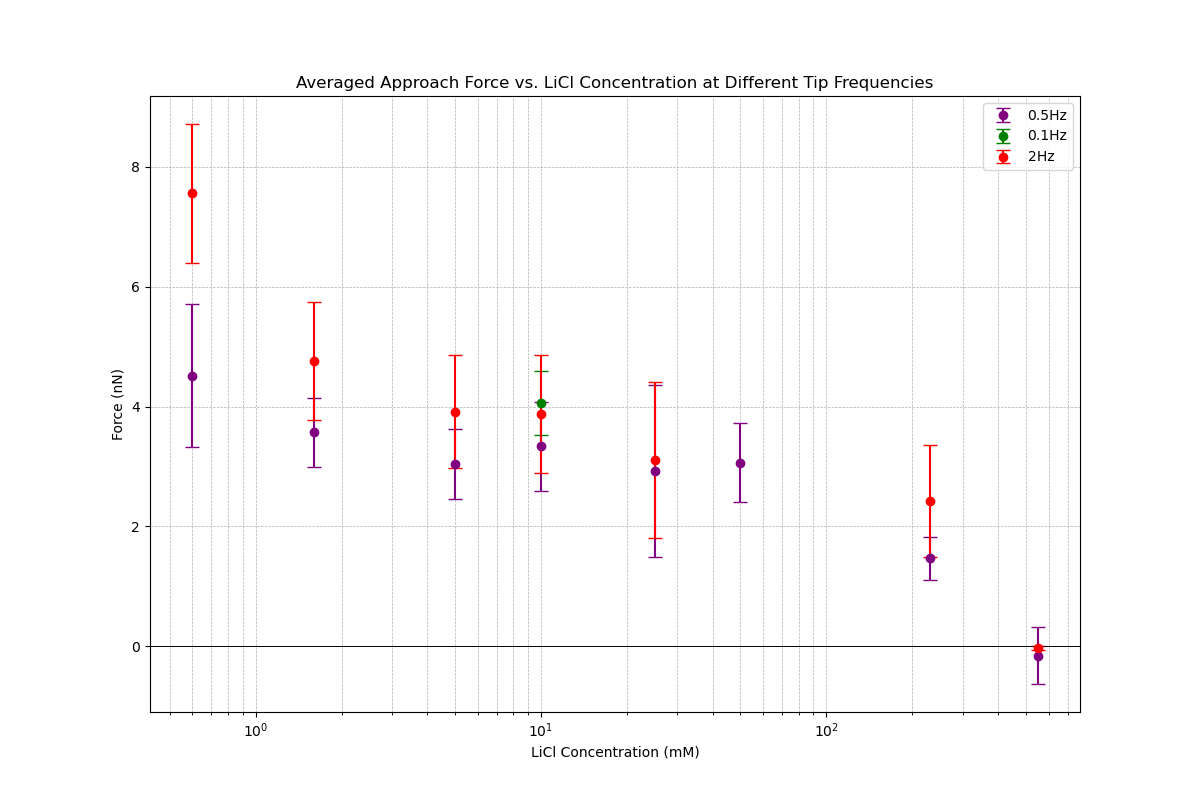
\includegraphics[width=\textwidth]{chapter7/Tip speed/Overall graph approach.png}
\caption{Averaged approach curve with the range of tip speeds. 0.5Hz represents the standard dataset, whereas 0.1Hz and 2Hz represent the modified speeds under investigation.}
\label{fig:ApproachAverageSpeed}
\end{figure}

The approach curve ($Figure \ref{fig:ApproachAverageSpeed}$) demonstrates an interesting observation: While minor, the increase in tip speed seems to indicate that the force required to bring the tip in contact increases with the speed of the tip. Possibly indicating that the system relaxes or changes in response to an approaching surface. 0.6mM is particularly interesting - as there was a significant increase in repulsive force at the higher speed, potentially indicating that tip speed has larger effects at very low ionic concentrations. 550mM is also interesting, where there was very little in the way of variation, and the approach force was nearly 0, potentially indicating that as the tip approaches, the surface was unable to relax in this way. 0.1Hz, while interestingly overlaps with the 2Hz datapoint, does not represent enough datapoints to fully make any solid conclusions. 

\begin{figure}[h!]
\centering
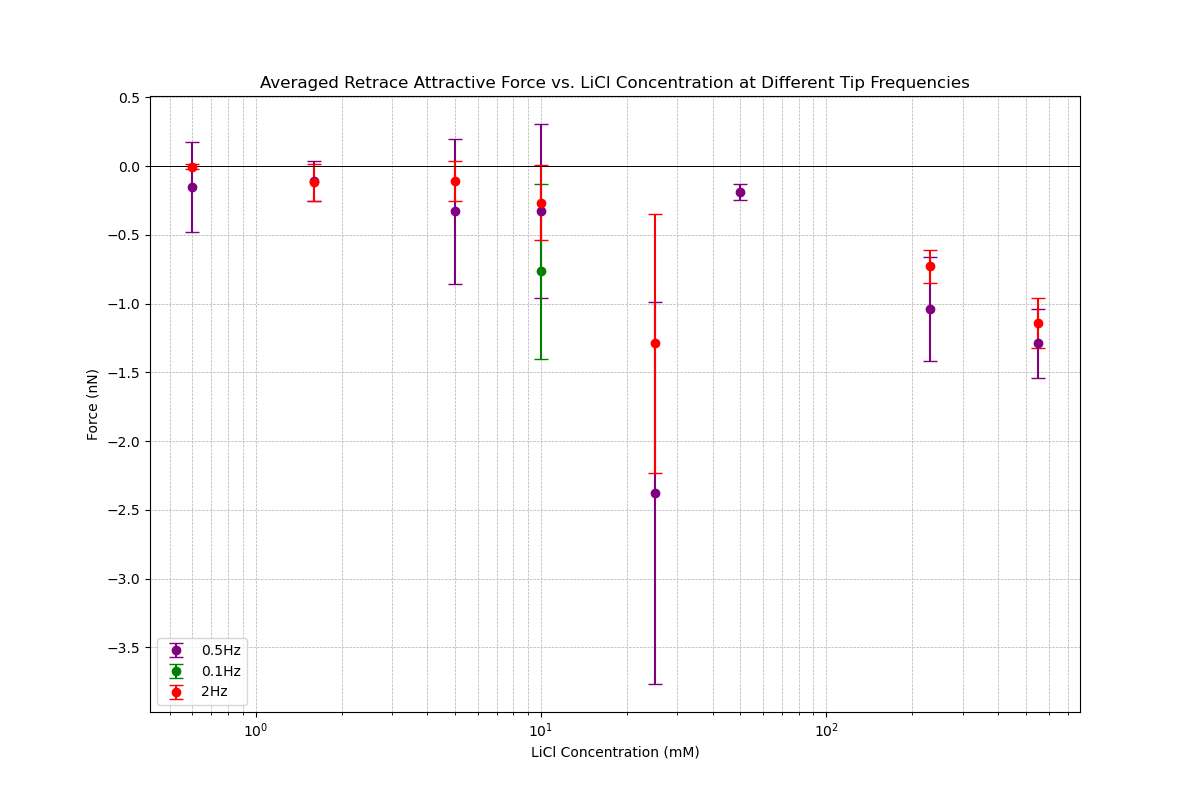
\includegraphics[width=\textwidth]{chapter7/Tip speed/Overall graph retrace.png}
\caption{Averaged retract curve with the range of tip speeds. 0.5Hz represents the standard dataset.}
\label{fig:RetractAverageSpeed}
\end{figure}

The retrace curve ($Figure \ref{fig:RetractAverageSpeed}$ shows a similar story - the majority of each of the datapoints are slightly less attracted to the surface, and as such, are easier to disengage. This again could indicate that the potential relaxation of the system to introduced conditions. 0.6mM as well does not seem to carry over the large change seen in the retrace curve, instead giving a value within expected ranges. The 0.1Hz datapoint, also seems to indicate that as tip speed decreases, the attractive potential between tip and surface increases. Another interesting factor is the 25mM datapoints; the wide range and intrigue of a sudden spike in attractive force is retained, if muted, in the data. However, for 25mM it is important to point out that the sites for 25mM values are the same between speeds, so if the cause is due to the site location themselves that would not be changed in this case.

Another aspect of investigation worth looking into is how the speed influences the reliability of the data. As tip speed increases, the volume of data decreases, as mentioned before, and as such it stands to reason that the standard deviation of the data would increase with this phenomena too.

\begin{figure}[h!]
\centering
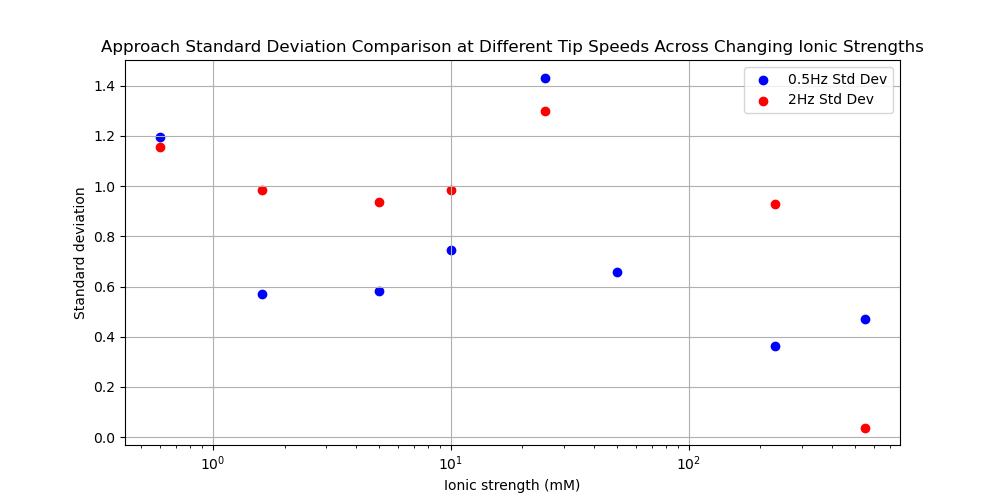
\includegraphics[width=\textwidth]{chapter7/Tip speed/Standard deviation change.png}
\caption{Averaged approach standard deviation between points. 0.5Hz represents the standard dataset.}
\label{fig:ApproachAverageSpeedDev}
\end{figure}

For the majority of the datapoints this theory proves true ($Figure \ref{fig:ApproachAverageSpeedDev}$, with 2 datapoints (0.6mM and 25mM) slightly below the slower value. The big exception however is the 550mM datapoint.

\begin{figure}[h!!!]
\centering
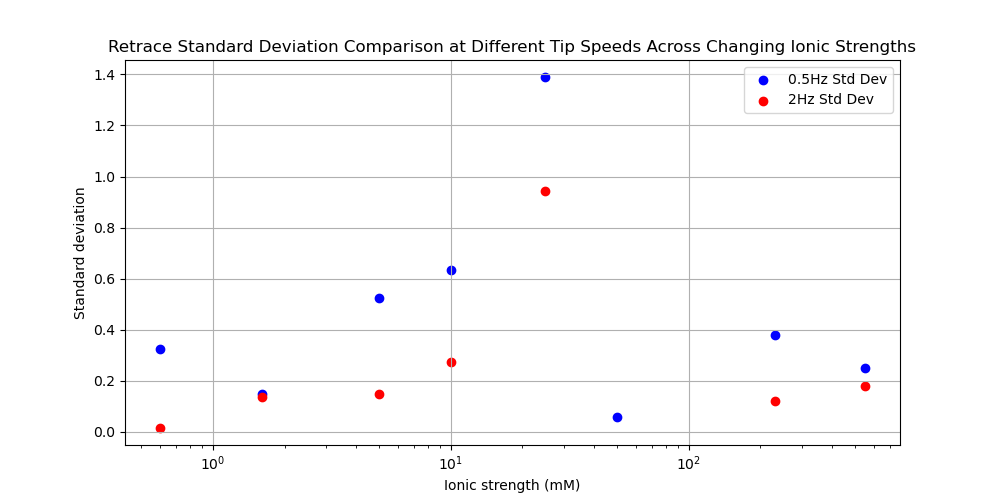
\includegraphics[width=\textwidth]{chapter7/Tip speed/Standard deviation change retract.png}
\caption{Averaged retract standard deviation between points. 0.5Hz represents the standard dataset.}
\label{fig:RetractAverageSpeedDev}
\end{figure}

However, when we consider the retract curve ($Figure \ref{fig:RetractAverageSpeedDev}$, our expectations are flipped. For each of the datapoints there is less variation between points, indicating a faster tip leads to a more stable analysis for the retraction. This could potentially lean into the relaxation theory, where, because there is less time for the system to relax and alter, the retrace experiences a more repeatable environment.

The other question that is raised by this analysis is thus, if a tip is held in constant and allowed to relax, how would that affect the results? This leads us directly into our next section, the dwell time analysis.

\section{Dwell time}

The dwell time represents the time in which the tip is held down onto the surface between the approach and retrace curves. This is usually done by the system attempting to use the feedback mechanism to keep the force applied to the tip at a constant force. This action was done for each and every curve taken on the machine for the dwell dataset.

For this series of data, only one point per concentration was done. This was due to the increased strain this often puts on the cantilever, which was an important and managed resource throughout this investigation. Overindulgence in certain aspects of the experimental protocol may lead to underindulgence or lack of exploration in other areas. As a result, a series of repeats could be performed to improve this analysis. For this case, the single dwell datapoints were compared against the averaged standard dataset points.

One other frustration seen during this operational mode was the inconsistency in data shape. This made using the analysis software particularly challenging, and is an area of potential improvement for the script. The script expects the user to provide a clear series of data with an approach and retrace aspect separated clearly, however, due to the 5 second dwell time providing a high degree of variability in forces, this can often trip up the detection method used to differentiate between the two phases. While two datapoints where successfully analysed using the script (25mM and 230mM) the other datapoints would've required a significant rewrite. As such, a simplified script was written to extract the peak force from the retrace curve, as, in theory, the only portion of the curve affected should be the retrace due to the potential impact of dwelling only being felt during the retrace curve.

\begin{figure}[h!]
\centering
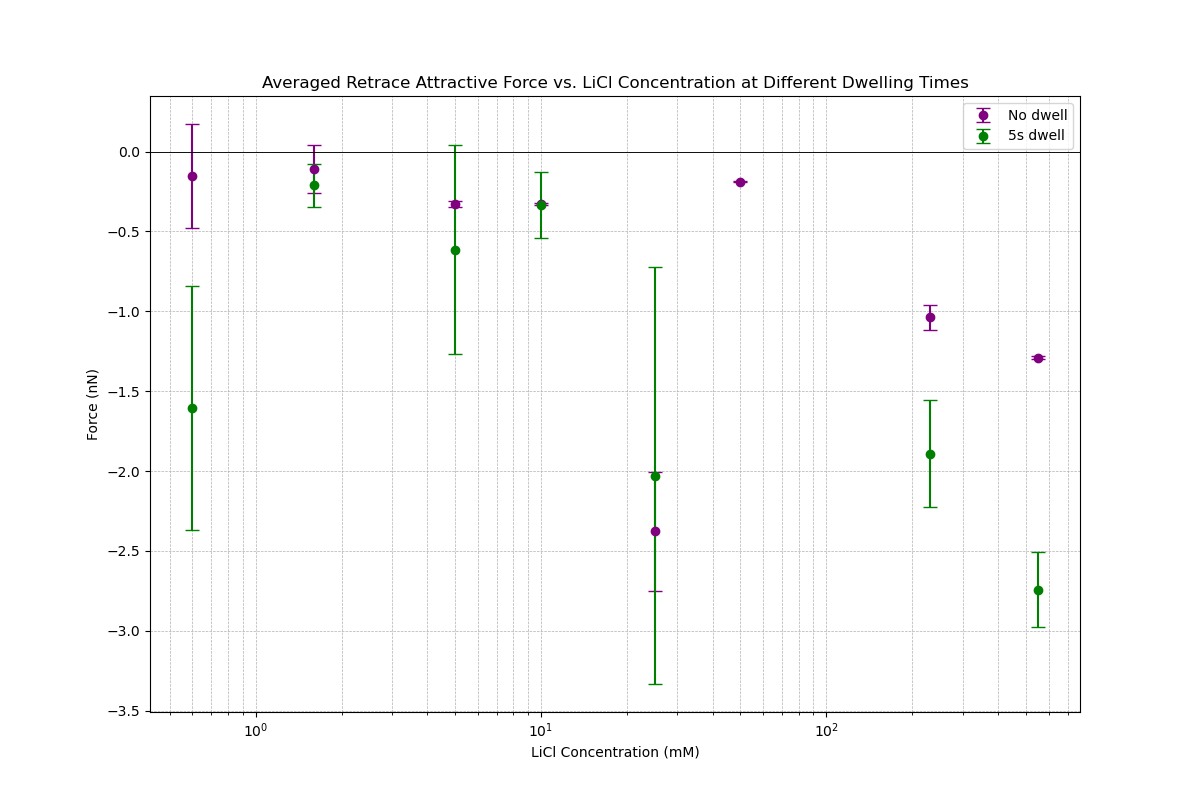
\includegraphics[width=\textwidth]{chapter7/Dwell/Retrace overall.png}
\caption{A graph demonstrating the averaged retract forces felt by the AFM tip at different LiCl concentrations with 5s dwell time and 0s dwell time respectively.}
\label{fig:RetractDwell}
\end{figure}

The retrace curve presents ($Figure \ref{fig:RetractDwell}$ an interesting but not unexpected conclusion: As tip exposure time increases, so too does the retentive force between the surface and tip on the retrace motion for some of the data points (0.6mM, 230mM and 550mM particularly). However, one that significantly stands out is 25mM, where the postulation is inverse. This could potentially be due to the previously proposed relaxation time, or because 25mM is consistently weird.

\begin{figure}[h!]
\centering
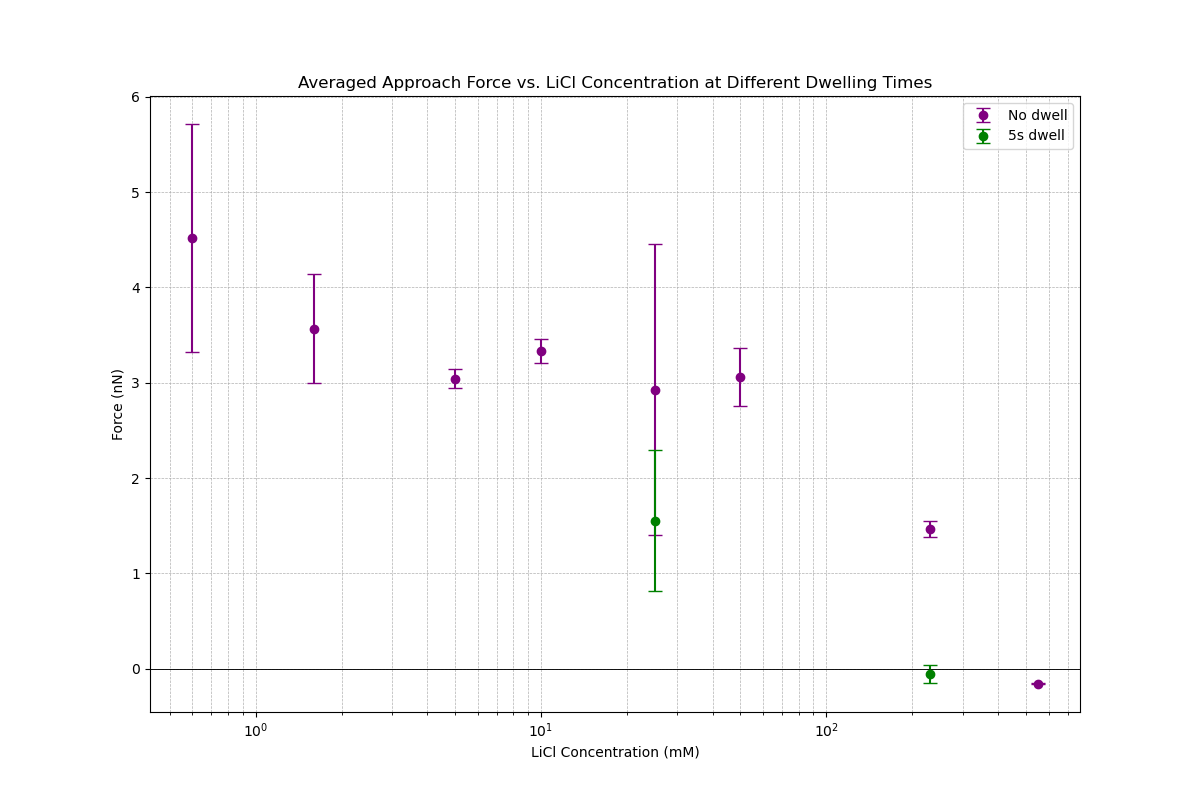
\includegraphics[width=0.95\textwidth]{chapter7/Dwell/Approach overall.png}
\caption{A graph demonstrating the averaged approach forces felt by the AFM tip at different LiCl concentrations with 5s dwell time and 0s dwell time respectively.}
\label{fig:ApproachDwell}
\end{figure}

However, when we look at the approach curve for the 2 points (figure \ref{fig:ApproachDwell}, we see an interesting picture. As the dwell time is increased, the time between curves is increased too, providing more time for water molecules and ions to adapt to the approaching tip, thus decreasing the repulsive force. This highlights that there is potentially hysteric effects.

\newpage
\section{pH analysis}

The pH level of a solution can significantly affect the forces between silica particles in a 50:50 water-glycerol solution due to changes in the surface charge of the silica particles. At different pH levels, the degree of ionization of silanol groups on the silica surface can vary, which impacts the electrostatic component of the total interparticle force. 

Silica surfaces are known to have silanol groups that can either accept or donate protons depending on the pH. At pH 5, which is close to the isoelectric point of silica, the surface charge density is reduced. This condition is interesting for force measurements since the electrostatic repulsion between particles is minimized, allowing other forces (such as van der Waals or steric forces) to be more prominently observed. \cite{Pavan2019}

While the solutions used in the standard dataset was around pH 7 on creation the pH can drift to slightly acidic due to carbon dioxide (CO\textsubscript{2}) from the air dissolving in the water, forming carbonic acid (H\textsubscript{2}CO\textsubscript{3}), which can dissociate to form bicarbonate (HCO\textsubscript{3}\textsuperscript{-}) and hydrogen ions (H\textsuperscript{+}). Though this effect is generally quite small, it is worth investigating to see if changes in pH could've altered the resulting dataset.

For this analysis a solution made up to pH of 5 instead of the standard pH 7 was performed, with the results directly compared against the 0.6mM LiCl concentration solution. 

\begin{figure}[h!]
\centering
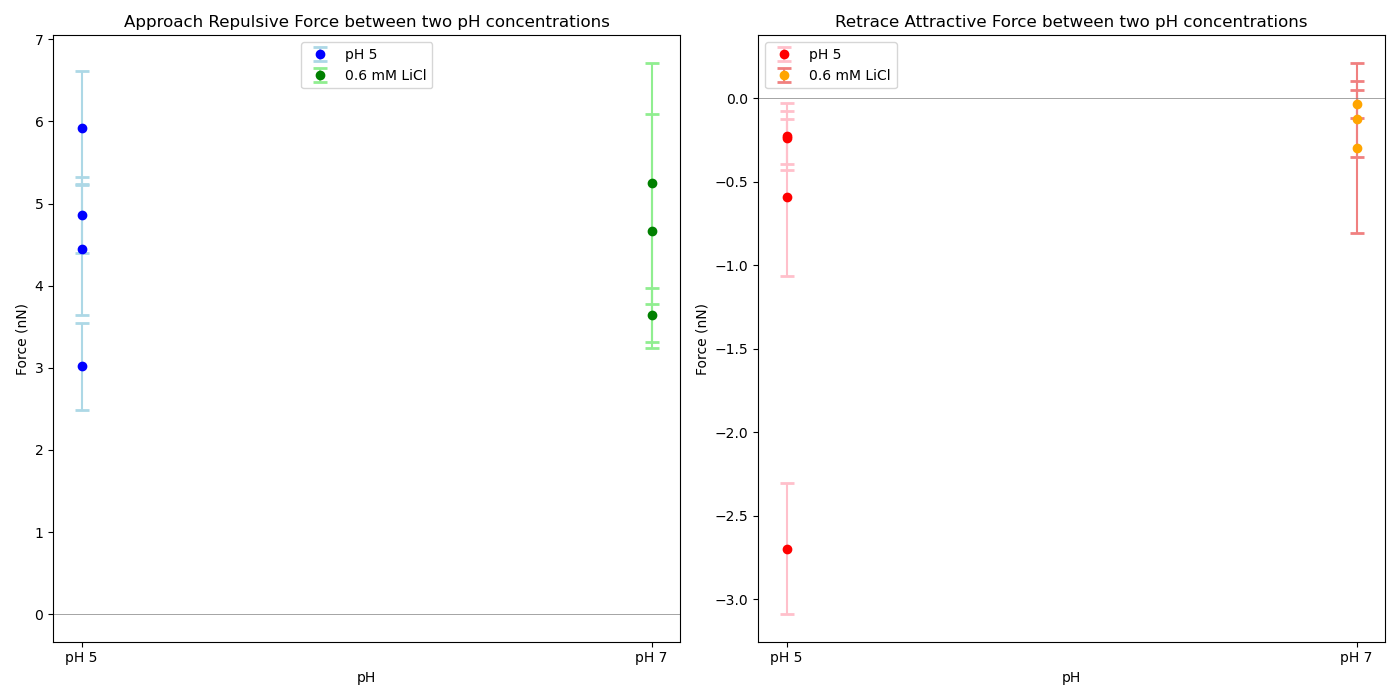
\includegraphics[width=\textwidth]{chapter7/pH/Overall image.png}
\caption{A graph demonstrating the differences in approach and retract forces at differing pHes. pH 5 is the deviation and pH 7 is the standard.}
\label{fig:pHOverall}
\end{figure}

From the observed change in pH, the resulting forces are similar to what would be expected with a pH 7 enviroment (0.6mM LiCl), with a striking overlap between the two data series on approach. The only observable difference between the two is in the retrace curve, where one datapoint is significantly more attractive. 

\newpage
\section{JPK Forcemapping}

One of the limitations of using the interpretation software is that it assumes that all curves are of the same shape. This is not the case for a range of sites. While this helps highlight features (such as the shelf) across multiple repeats on the same area, it does not take into account a range of different sites. That being said, however, as long as the user does not attempt to use the software incorrectly to provide an averaged graph, the attractive/repulsive force analysis is perfectly applicable and as such was used to analyse each induvidual curve from the forcemapping.

Due to the differences between the AFMs, and potentially the way the AFMs were used to measure the interactions, the ``shelf" seen was more of a snap to contact point in the curve. This meant that the shelf seen in the previous AFM, may have been the point in which the tip snapped to the surface, and the older AFM may not have been able to detect or measure this sudden change in the way the new one has. 

Due to the limited window in which this AFM was available, it was not possible to explore this interaction further, but it is promising that this shelf feature is present across multiple AFMs and sites. The script was adapted in order to use the new data type, with a specialised script written to convert exportable JPK filetypes into the format expected by the software.

The operation of the AFM was done with the same tip and conditions, with a 16x16 grid with a 1um distance between each of the sites. Only 2 concentration could be performed during the available time: 0.6mM and 10mM.

\subsubsection{0.6mM approach}

As the script is written to concatenate a range of graphs into a single one, there were some quirks of processing. For one, the histogram shows a range of forces, but it is important to know that for this range it is across different areas of the glass, rather than a single area.

% Approach f c hist
\begin{figure}[h]
    \centering
    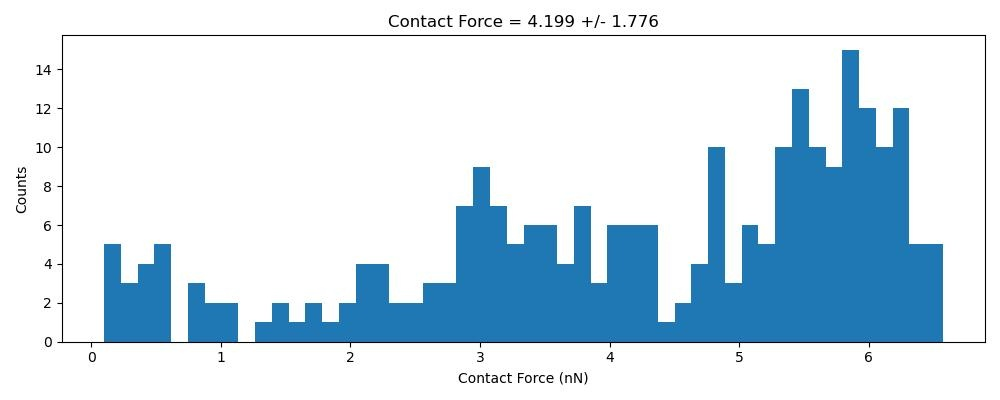
\includegraphics[width=0.8\textwidth]{chapter7/ForceMaps/0.5mM/approach_f_c_hist.jpg}
    \caption{Approach force histogram for 0.5mM concentration.}
    \label{fig:approach_f_c_hist_0.5mM}
\end{figure}

% Approach df zp bin
%\begin{figure}[h]
%    \centering
%    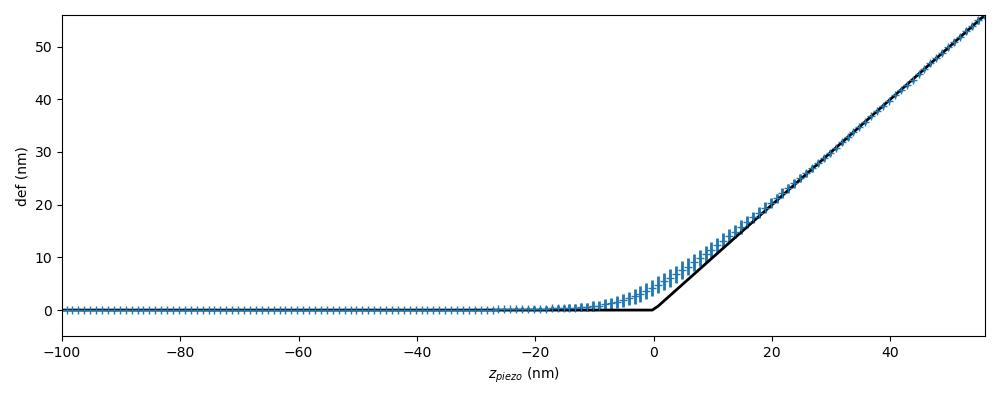
\includegraphics[width=\textwidth]{chapter7/ForceMaps/0.5mM/approach_df_zp_bin.jpg}
%    \caption{Approach df zp bin for 0.5mM concentration.}
%    \label{fig:approach_df_zp_bin_0.5mM}
%\end{figure}

% Approach heatmap
\begin{figure}[h]
    \centering
    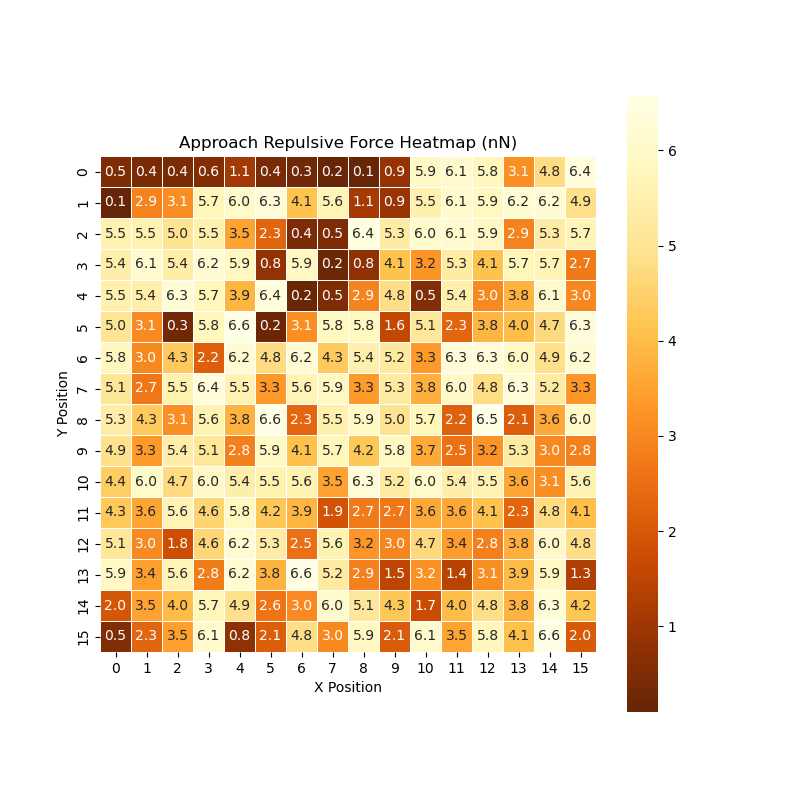
\includegraphics[width=\textwidth]{chapter7/ForceMaps/0.5mM/Approach heatmap.png}
    \caption{Approach heatmap for 0.5mM concentration.}
    \label{fig:approach_heatmap_0.5mM}
\end{figure}

The heatmap demonstrates the wide range of variability seen on a glass surface. This indicates that interacting surfaces is significantly dependent on local conditions of the surface. A range of forces is present, indicating variability in the interaction forces across different points on the surface. This could be due to surface heterogeneities or variations in local chemical composition and structure. 
\newpage

\subsubsection{0.6mM retract}

However for the retraction portion of the curve, the histogram shows the distribution of attractive forces measured during the retract phase across all different sites. Most measurements cluster around a relatively small attractive force as seen in the standard dataset, but there is an outlier showing a strong attraction. This suggests that while the retract forces are generally consistent, certain specific interactions result in much stronger attraction. 

% Retract f a hist
\begin{figure}[h!!!]
    \centering
    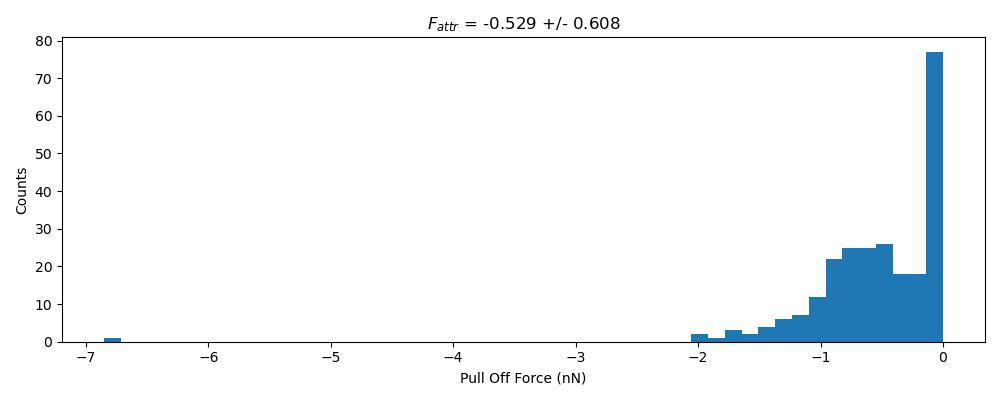
\includegraphics[width=0.8\textwidth]{chapter7/ForceMaps/0.5mM/retract_f_a_hist.jpg}
    \caption{Retract force histogram for 0.5mM concentration.}
    \label{fig:retract_f_a_hist_0.5mM}
\end{figure}

% Retract heatmap
\begin{figure}[h!!!]
    \centering
    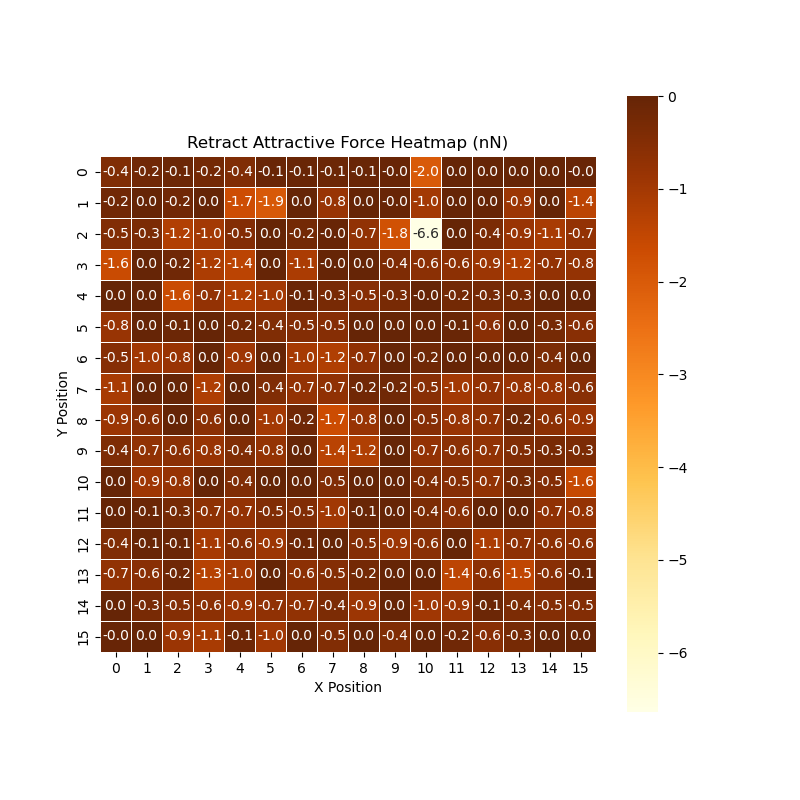
\includegraphics[width=0.8\textwidth]{chapter7/ForceMaps/0.5mM/Retract heatmap.png}
    \caption{Retract heatmap for 0.5mM concentration.}
    \label{fig:retract_heatmap_0.5mM}
\end{figure}

% Retract df zp bin
%\begin{figure}[h]
%    \centering
%    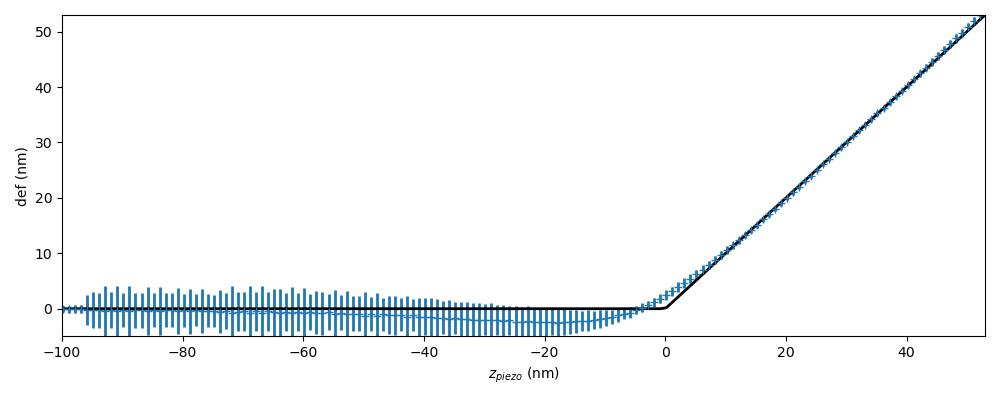
\includegraphics[width=\textwidth]{chapter7/ForceMaps/0.5mM/retract_df_zp_bin.jpg}
%    \caption{Retract df zp bin for 0.5mM concentration.}
%    \label{fig:retract_df_zp_bin_0.5mM}
%\end{figure}



\newpage
\subsubsection{10mM approach}

The histogram shows a wide range of contact forces with a relatively large standard deviation. This suggests that at the 10mM concentration, there is a significant variability in the forces measured across different sites of the surface during the approach phase. Interestingly, for some curves an attractive force was observed which is unlike the standard dataset. The attractive part of the curves are generally clustered towards the top of the heatmap suggesting that the surface has regions of varying repulsive forces. 

\begin{figure}[h!!!]
    \centering
    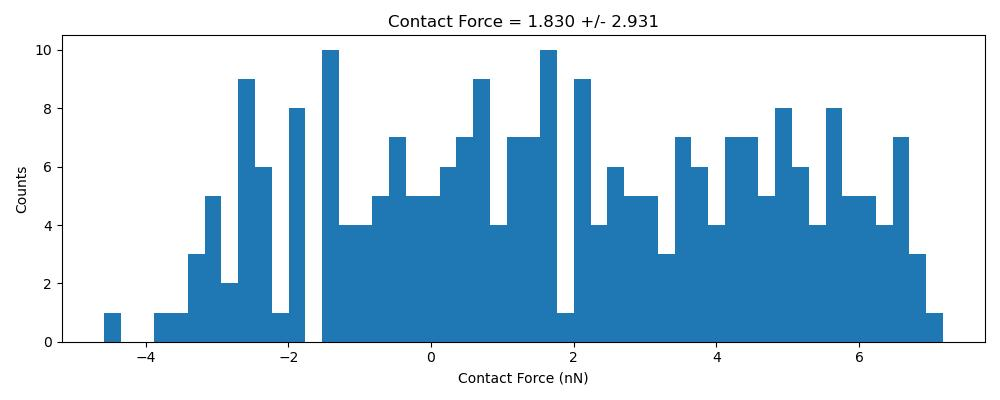
\includegraphics[width=0.7\textwidth]{chapter7/ForceMaps/10mM/approach_f_c_hist.jpg}
    \caption{Retract heatmap for 0.5mM concentration.}
    \label{fig:appro_fc_10mM}
\end{figure}

% Approach heatmap
\begin{figure}[h!!!!!]
    \centering
    \includegraphics[width=0.75\textwidth]{chapter7/ForceMaps/10mM/Approach heatmap.png}
    \caption{Approach heatmap for 10mM concentration.}
    \label{fig:approach_heatmap_10mM}
\end{figure}

\newpage
\subsubsection{10mM retract}

The retract portion of the curve is even more unusual with a consistent attractive force recorded at about 34nN. This is unlike anything else seen in the dataset, so it is likely that the tip was contaminated or damaged, especially since the tip used was a reused one at the time.

\begin{figure}[h!!!]
    \centering
    \includegraphics[width=0.79\textwidth]{chapter7/ForceMaps/10mM/contact_force_histogram.png}
    \caption{Retract heatmap for 0.5mM concentration.}
    \label{fig:contfhist}
\end{figure}

\begin{figure}[h!]
\centering
\includegraphics[width=0.7\textwidth]{chapter7/ForceMaps/10mM/Retract_heatmap.png}
\caption{Retract heatmap for 10mM concentration.}
\label{fig:pHOverall}
\end{figure}

While the 10mM results are ultimately suspicious, it does highlight the variability seen in these kinds of surfaces. As to what could possibly cause these high degrees of variability, that leads us to the next chapter: the overall analysis of all of the data presented so far.
